\documentclass[tikz]{standalone}

\begin{document}
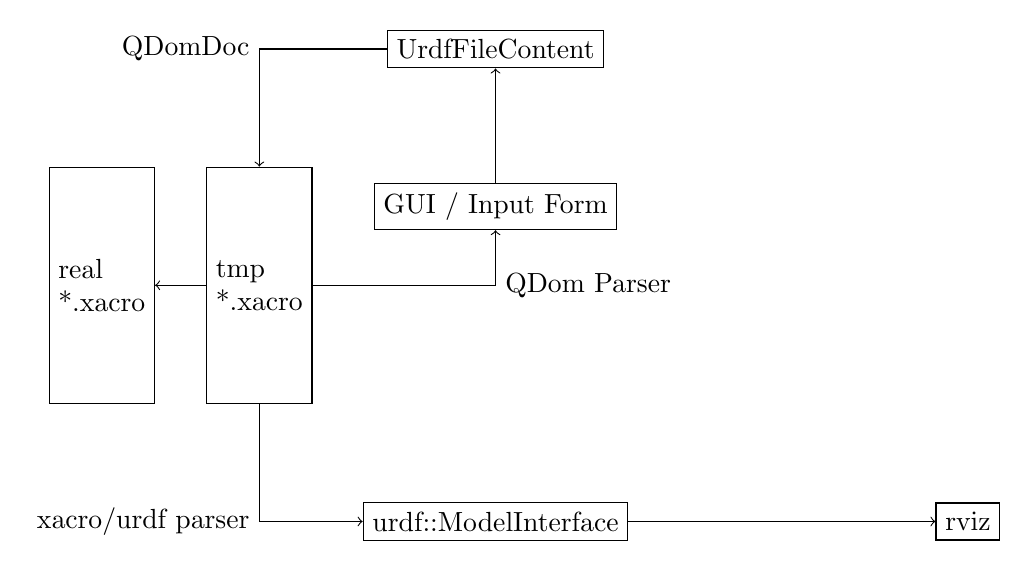
\begin{tikzpicture}


\path (0,0) node[draw, align=left, minimum height=3cm](tmpXacro){tmp \\ *.xacro};
\path (-2,0) node[draw, align=left, minimum height=3cm](xacro){real \\ *.xacro};
\path (3,-3) node[draw, align=left](urdf){urdf::ModelInterface};
%\path (6,0) node[draw, align=left](model){RobotDescriptionModel};
\path (9,-3) node[draw, align=left](rviz){rviz};
\path (3,3) node[draw, align=left](fileManager){UrdfFileContent};
\path (3,1) node[draw, align=left](gui){GUI / Input Form};



\draw[->] (tmpXacro) -- (xacro);
\draw[->] (tmpXacro) |- (urdf)node[midway, left]{xacro/urdf parser};
%\draw[->] (urdf) -| (model)node[midway, right]{updateRobotModel};
%\draw[<->] (model) -|(gui);
\draw[->] (tmpXacro) -| (gui)node[midway, right]{QDom Parser};
\draw[->] (fileManager) -| (tmpXacro)node[midway, left]{QDomDoc};
\draw[->] (gui) -- (fileManager)node[midway, right]{};
\draw[->] (urdf) --(rviz);


\end{tikzpicture}
\end{document}